%%%%%%%%%%%%%%%%%%%%%%% CHAPTER - 1 %%%%%%%%%%%%%%%%%%%%\\
\chapter{Introduction}
\label{C1} %%%%%%%%%%%%%%%%%%%%%%%%%%%%
\graphicspath{{Figures/Chapter-1figs/PDF/}{Figures/Chapter-1figs/}}
% \noindent\rule{\linewidth}{2pt}
\onehalfspacing
% \setlength{\parskip}{24pt}
\textit{This Chapter provides...... }
%%%%%%%%%%%%%%%%%%%%%%%%%%%%%%%%%%%%%%%%%%%%%%%%%%%%%%%%%%%%%%%%%%%%%%%%%%%%%%%%%%%%%%%%%%%%%%%%%%%%%%%%%%%%%%%%%%%%%%%%%%%%%%%%%%%%%%
\thispagestyle{empty}
%%%%%%%%%%%%%%%%%%%%%%%%%%%%%%%%%%%%%%%%%%%%%%%%%%%%%%%%%%%%%%%%%%%%%%%%%%%%%%%%%%%%%%%%%%%%%%%%%%%%%%%%%%%%%%%%%%%%%%%%%%%%%%%%%%%%%%
\section{Background} \label{S1.1}
Type introduction part here. \cite{whygaussianity}
%%%%%%%%%%%%%%%%%%%%%%%%%%%%%%%%%%%%%%%%% Figure 1 %%%%%%%%%%%%%%%%%%%%%%%%%%%%%%%%%%%%%%%%%%%%%%%%%%%%%%%%%%%%%%%%%%%%%%%%%%%%%%%%%%%%
\begin{figure}[b!]
	\center	
	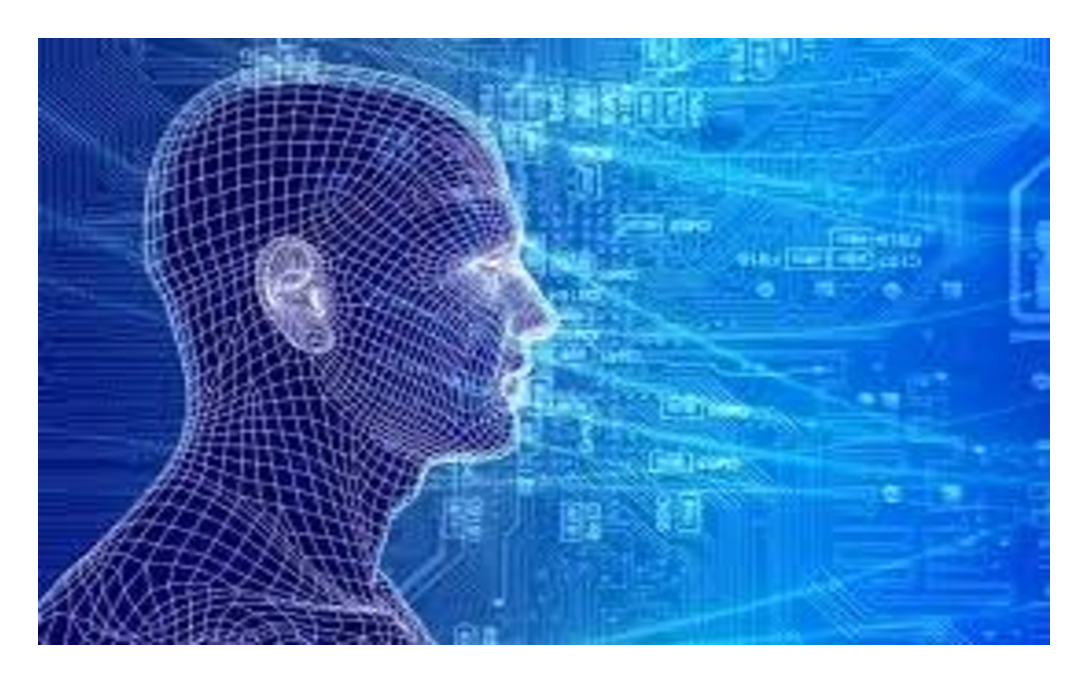
\includegraphics[scale=0.7]{fig1_1} 	
	\caption{abcdefgh} 
	\label{f1.1}	
\end{figure}  
%%%%%%%%%%%%%%%%%%%%%%%%%%%%%%%%%%%%%%%%%%%%%%%%%%%%%%%%%%%%%%%%%%%%%%%%%%%%%%%%%%%%%%%%%%%%%%%%%%%%%%%%%%%%%%%%%%%%%%%%%%%%%%%%%%%%%%%

%%%%%%%%%%%%%%%%%%%%%%%%%%%%%%%%%%%%%%%%%%%%%%%%%%%%%%%%%%%%%%%%%%%%%%%%%%%%%%%%%%%%%%%%%%%%%%%%%%%%%%%%%%%%%%%%%%%%%%%%%%%%%%%%%%%%%%%
\section{Motivation for the present research work} \label{S1.2} 
Type motivation here.
\section{Problem statement} \label{S1.3}
 Type Problem statement here.

 Given a set of numbers, there are elementary methods to compute 
its \acrlong{gcd}, which is abbreviated \acrshort{gcd}. This process 
is similar to that used for the \acrfull{lcm}.

\clearpage

\printglossary[type=\acronymtype]
%%%%%%%%%%%%%%%%%%%%%%%%%%%%%%%%%%%%%%%%%%%%%%%%%%%%%%%%%%%%%%%%%%%%%%%%%%%%%%%%%%%%%%%%%%%%%%%%%%%%%%%%%%%%%%%%%%%%%%%%%%%%%%%%%%%%%%%

\section{Organization of the thesis} \label{S1.4}
The research work presented in the thesis is organized and structured in the form of seven chapters, which are briefly described as follows:
\begin{enumerate}[label=\textbf{\roman*)}]
	\item \textbf{Chapter 1} describes the ......................................
	\item \textbf{Chapter 2} provides a comprehensive review of ...................................
	\item \textbf{Chapter 3} presents a .................................
	\item \textbf{Chapter 5} deals with ............................................
	\item \textbf{Chapter 6} presents a ...............................................
	\item \textbf{Chapter 7} concludes the thesis with overall discoveries of the present research work. The scope for future work is also mentioned. 
\end{enumerate} 
